\chapter{The Experimental Apparatus}
\section{The Large Hadron Collider}
The Large Hadron Collider (LHC) is a particle accelerator designed to explore the physics of particles at the energy scale of electroweak symmetry breaking. The accelerator occupies a 26.7 km tunnel beneath the Switzerland-France border near Geneva, which previously housed the Large Electron Positron Collider (LEP). Protons are accelerated in two counter-rotating beams up to a design momentum of $7~\mbox{TeV}/c$. The beams collide at four interaction points (IPs), shown in figure~\ref{fig:LHC-IPs}, where four collider detectors, ATLAS, CMS, LHCb, and ALICE, analyze the remnants of the collisions.

\begin{figure}[htbp]
	\centering
	\resizebox{0.4\textwidth}{!}{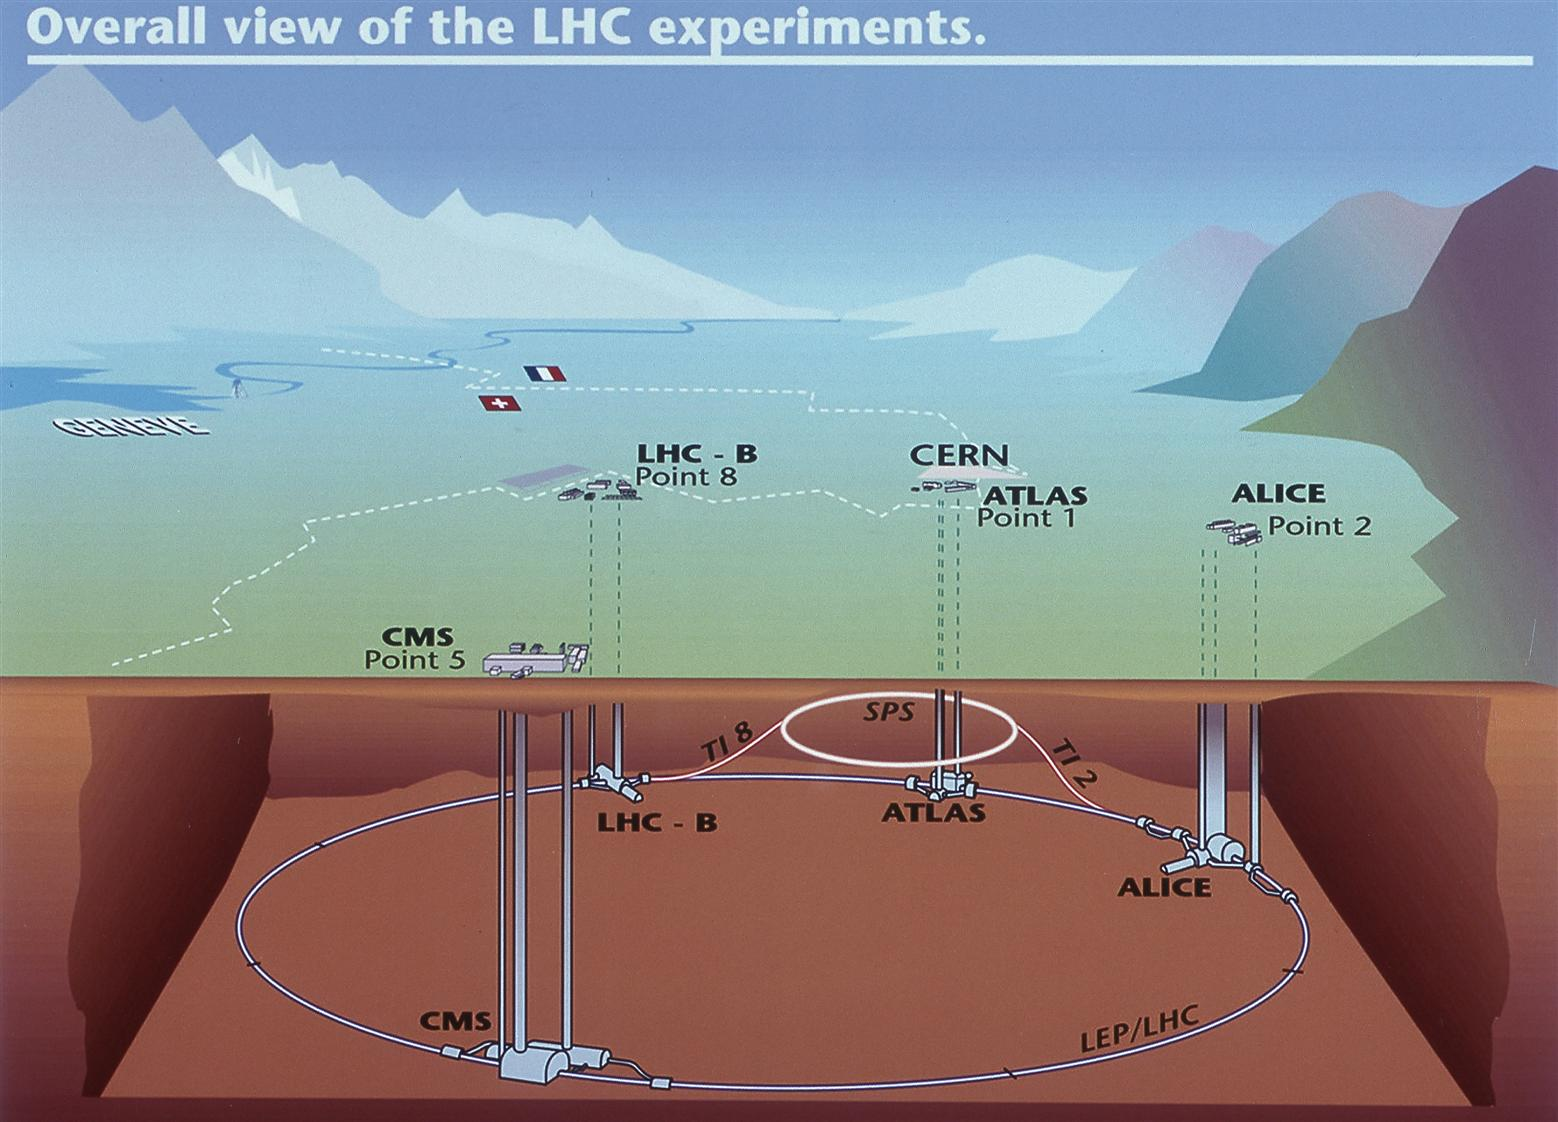
\includegraphics{figures/ch3-experiment/LHC_IPs}}
	\caption{The LHC and the four interaction points where the beams are brought into collision. The ATLAS experiment is located at interaction point 1.}
	\label{fig:LHC-IPs}
\end{figure}


The LHC project was approved in 1994 by the CERN Council, and construction proceeded over the ensuing 14 years. The collider detectors were constructed in parallel, beginning with the excavation of two additional caverns at IP1 and IP5 for the ATLAS and CMS detectors (LHCb and ALICE occupied the existing caverns at IP2 and IP8, which previously housed the DELPHI and L3 LEP experiments). The first beam was circulated on 10 September 2008; however, on 19 September, the LHC sustained severe damage due to an incident stemming from a faulty joint between magnets\footnote{A postmortem analysis implicated a bad splice between the superconducting cables of adjacent magnets as the source of the incident, with a resistance about $10^3$ times above specification. The joint melted, and 275~MJ of energy in the magnets dissipated in electric arcs, which vaporized beam pipes and breached the cryogenic vessel containing the magnets. A large amount of liquid helium entered the vacuum vessel and heated rapidly, breaking several vacuum barriers of the cryostats with a force of up to 56 tons. Ultimately, 30 dipoles and 7 quadrupoles were damaged beyond repair, and another 9 dipoles and 7 quadrupoles required repairs; 9 magnet interconnections were destroyed; 26 magnets were pushed down the tunnel; 276~MJ of energy were dissipated in electrical faults and arcs; 6 tons of helium were lost; and 2.8~km of both beam pipes were contaminated with fragments of insulation, with 1~km also contaminated with soot from molten copper and insulation.~\cite{Rossi:2010el}}. Repairs took an extra year, and the energy of the beams was reduced to $3.5-4~\mbox{TeV}$ for the first data-taking run, to mitigate the risk of another possible faulty joint. 

Proton-proton collisions at a center-of-mass energy of $\sqrt{s}=7~\mbox{TeV}$ commenced in early 2010. The LHC delivered an integrated luminosity of $\int L dt=48.1~\mbox{pb}^{-1}$ to the ATLAS detector in 2010, and $\int L dt=5.46~\mbox{fb}^{-1}$ in 2011. In 2012, the collision energy was increased to $\sqrt{s}=8~\mbox{TeV}$, and a dataset of $\int L dt=22.8~\mbox{fb}^{-1}$ was delivered. 

\subsection{Accelerator Components}
The primary devices used for acceleration are synchrotrons, made up of a variety of magnets and radio frequency (RF) cavities. The magnets are used to manipulate the particle beams: dipole magnets are used for bending the beams in a circle and for steering the beams down transfer lines between the accelerators, while quadrupole and higher moment magnets are used to focus the beams. RF cavities are metallic structures used for particle acceleration. The RF cavities are driven by klystrons, radio frequency amplifiers that act as power sources, at their resonant frequency, creating an oscillating electric field inside the structure. The frequency of the RF cavities is matched to the rotation frequency of the particle beams.

The RF oscillations result in the particle beam bunching into so-called RF buckets, shown schematically in figure~\ref{fig:RF-bucket}; the center of the bucket corresponds to particles with the reference energy (determined by the magnets) which experience no force in the RF cavities. During \emph{flat-top} operation, where the particle are held at fixed energy in the synchrotron, particles at the center of the RF bucket remain stationary at that point (neglecting energy losses due to synchrotron radiation), while nearby particles oscillate around the fixed point. During a \emph{ramp}, where particles are accelerated, the magnetic fields of the dipoles are slowly increased, shifting the RF bucket and causing the particle bunches to fall on the accelerating edge of the electric field oscillations. 

\begin{figure}[htbp]
	\centering
	\resizebox{0.5\textwidth}{!}{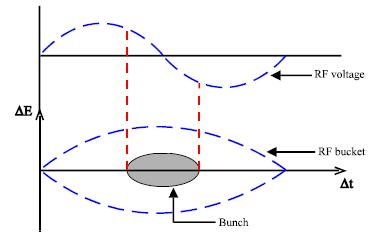
\includegraphics{figures/ch3-experiment/LHC_RF_buckets}}
	\caption{Schematic picture of an RF bucket. Particles at the center of the RF bucket experience no acceleration}
	\label{fig:RF-bucket}
\end{figure}

\clearpage

\subsection{The Accelerator Complex}

\underline{\textbf{Injection Chain}}

\begin{figure}[htbp]
	\centering
	\resizebox{3.5in}{!}{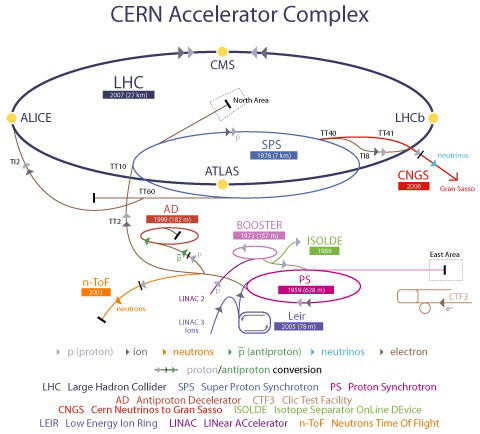
\includegraphics{figures/ch3-experiment/converted/LHC_accelerator_complex.png}}
	\caption{The LHC accelerator complex. The proton injection chain begins at LINAC2, proceeding through the booster, PS, and SPS before reaching the LHC. The facility also provides ions to the LHC, as well as a variety of particles to other experiments.}
	\label{fig:LHC-accelerator-complex}
\end{figure}


The LHC itself is the last stage of a chain of lower-energy accelerators, shown in figure~\ref{fig:LHC-accelerator-complex}. A full description of the injection chain can be found at~\cite{Benedikt:2004wm}. The staged acceleration chain allows for maintaining a high-quality beam over many decades of energy. It consists of a linear accelerator and three synchrotrons which were used for previous generations of experiments at CERN. The reuse of the older accelerators is economical while still meeting the stringent performance requirements of the LHC, providing up to 2808 proton bunches with a very small transverse emittance and controllable longitudinal emittance. 

Protons are produced from hydrogen gas using a duoplasmatron source, which strips electrons from protons in a high electric field. After passing through a $90~\mbox{kV}$ pre-injector, a radio frequency quadrupole (RFQ) focuses and accelerates the protons to $750~\mbox{kV}$. A linear accelerator (LINAC2) then accelerates the protons to $50~\mbox{MeV}$ using RF cavities. The protons then pass through an $80~\mbox{m}$-long transfer line into the the Proton Synchrotron Booster (PSB) and Proton Synchrotron (PS). 

The PSB consists of four stacked circular synchrotrons, $157~\mbox{m}$ in circumference, and accelerates the protons to $1.4 \GeV$. The use of four separate rings mitigates the space charge effects caused by the repulsion of protons within a bunch, which scale as $N_b/(\beta\gamma^2)$, where $N_b$ is the number of protons per bunch. The protons are then injected into single-ring PS, where the higher injection energy reduces the space charge effect. The RF cavities of the PS, operating at several frequencies, accelerate the beams to $26 \GeV$, and also split the protons into the bunches eventually inject into the LHC. Nominally, this yields 72 bunches separated by 25~ns, but for Run I, 50~ns spacing was used instead. 

The protons are extracted from the PS at intervals of 3.6~s and injected into the third synchrotron in the chain, the $7~\mbox{km}$-circumference Super Proton Synchrotron (SPS). Immediately prior to extraction, the bunches are rotated by increasing the RF voltage, reducing the longitudinal emittance in order to ease capture in the SPS RF buckets, which have a frequency of $200~\mbox{MHz}$.  Up to four PS batches are injected per SPS cycle, after which the particle are accelerated at an average of $78~\GeV/s$ to the LHC injection energy of $450 \GeV$. Flat-top is maintained for about one second, during which the injection is prepared:

\begin{itemize}
	\item The magnets used for the beam extraction are ramped, safety checks are performed, and the SPS phase is tuned to match that of the LHC.
	\item The bunch length is compressed using an RF voltage increase, as in the PS-SPS transfer.
	\item The tails of the bunches are removed, down to $3$--$3.5\sigma$.
\end{itemize}

The SPS cycle takes 21.6 seconds, leading to a total LHC filling time of about nine minutes.

\underline{\textbf{LHC Main Ring}}
The LHC main ring accelerates protons from the injection energy of $450 \GeV$ to the collision energy, $3.5 \TeV$ or $4 \TeV$ for proton-proton collisions during Run I. The 26.7~km ring consists of eight arcs and eight straight sections, shown in figure~\ref{fig:LHC-segments}. Each straight section is called an \emph{insertion region} (IR), and contain either collider experiments or important services. IRs 1, 2, 5, and 8 contain the ATLAS, LHCb, CMS, and ALICE experiments, respectively; IR 4 contains two independent $400~\mbox{MHz}$ RF systems, one for each of the counter-rotating beams; IR 6 contains the beam dump system; and IRs 3 and 7 contain collimation systems. The beams are contained in separate beam pipes except at the collision points.

\begin{figure}[htbp]
	\centering
	\resizebox{0.5\textwidth}{!}{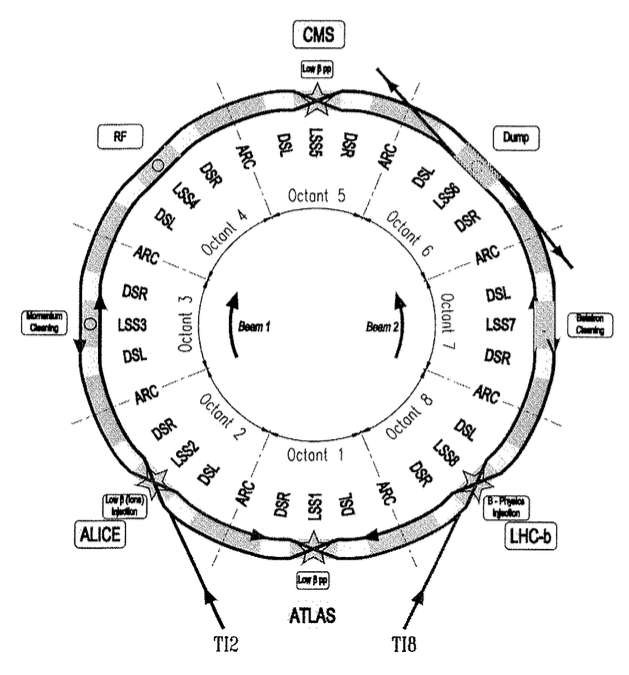
\includegraphics{figures/ch3-experiment/LHC_segments}}
	\caption{Layout of the LHC. The ring consists of eight arcs and eight long straight sections (LSS). Each junction between an arc and a LSS contains a dispersion suppressor cell (DSL, DSR). TI2 and TI8 are the two injection tunnels (``tunnel d'injection'') leading from the SPS to the LHC.}
	\label{fig:LHC-segments}
\end{figure}


The beams are controlled by over 7,000 magnets. The primary bending and focusing are performed by 1232 superconducting dipole and 392 superconducting quadrupole magnets. The dipole magnets, shown in figure~\ref{fig:LHC-dipole-magnets}, have a nominal field of $8.33~\mbox{T}$ and a length of $15~\mbox{m}$. The conducting coils are constructed from Nb-Ti Rutherford cables, and are cooled to $1.9~\mbox{K}$ using superfluid helium. The dipoles have a double-bore structure, providing the bending field for both beams. 

\begin{figure}[htbp]
	\centering
	\subfloat[] {
		\resizebox{0.45\textwidth}{!}{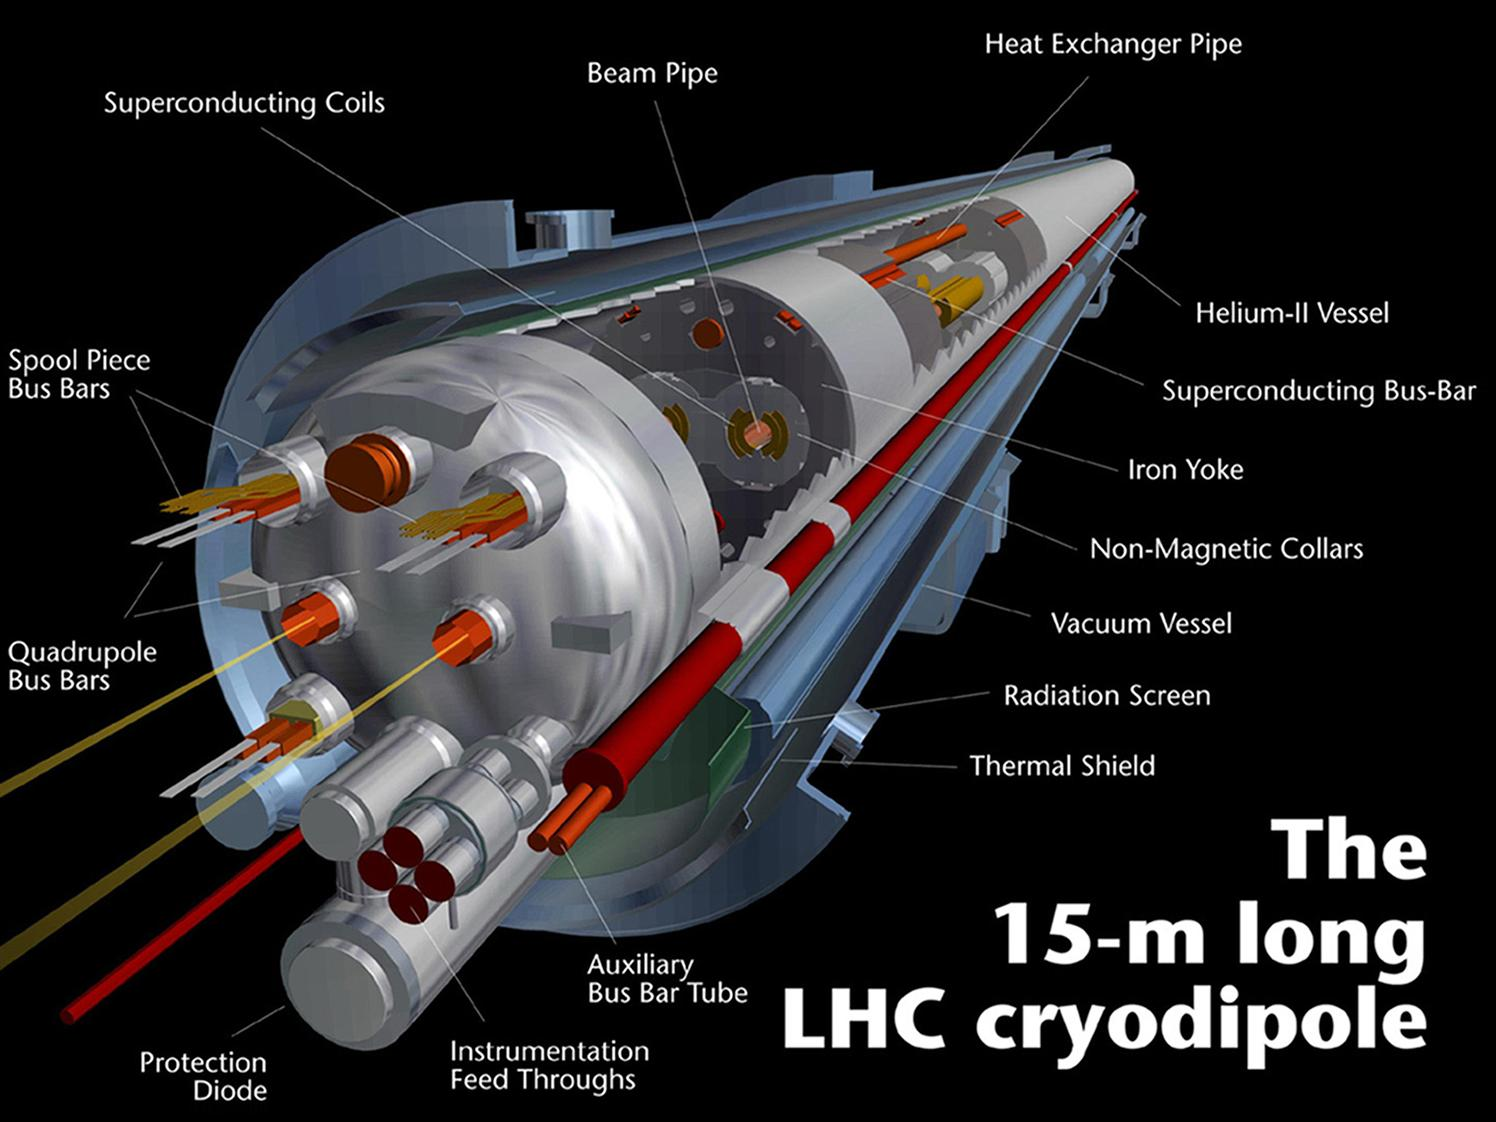
\includegraphics{figures/ch3-experiment/LHC_dipole_sketch}}
	}
	\hfill
	\subfloat[] {
		\resizebox{0.45\textwidth}{!}{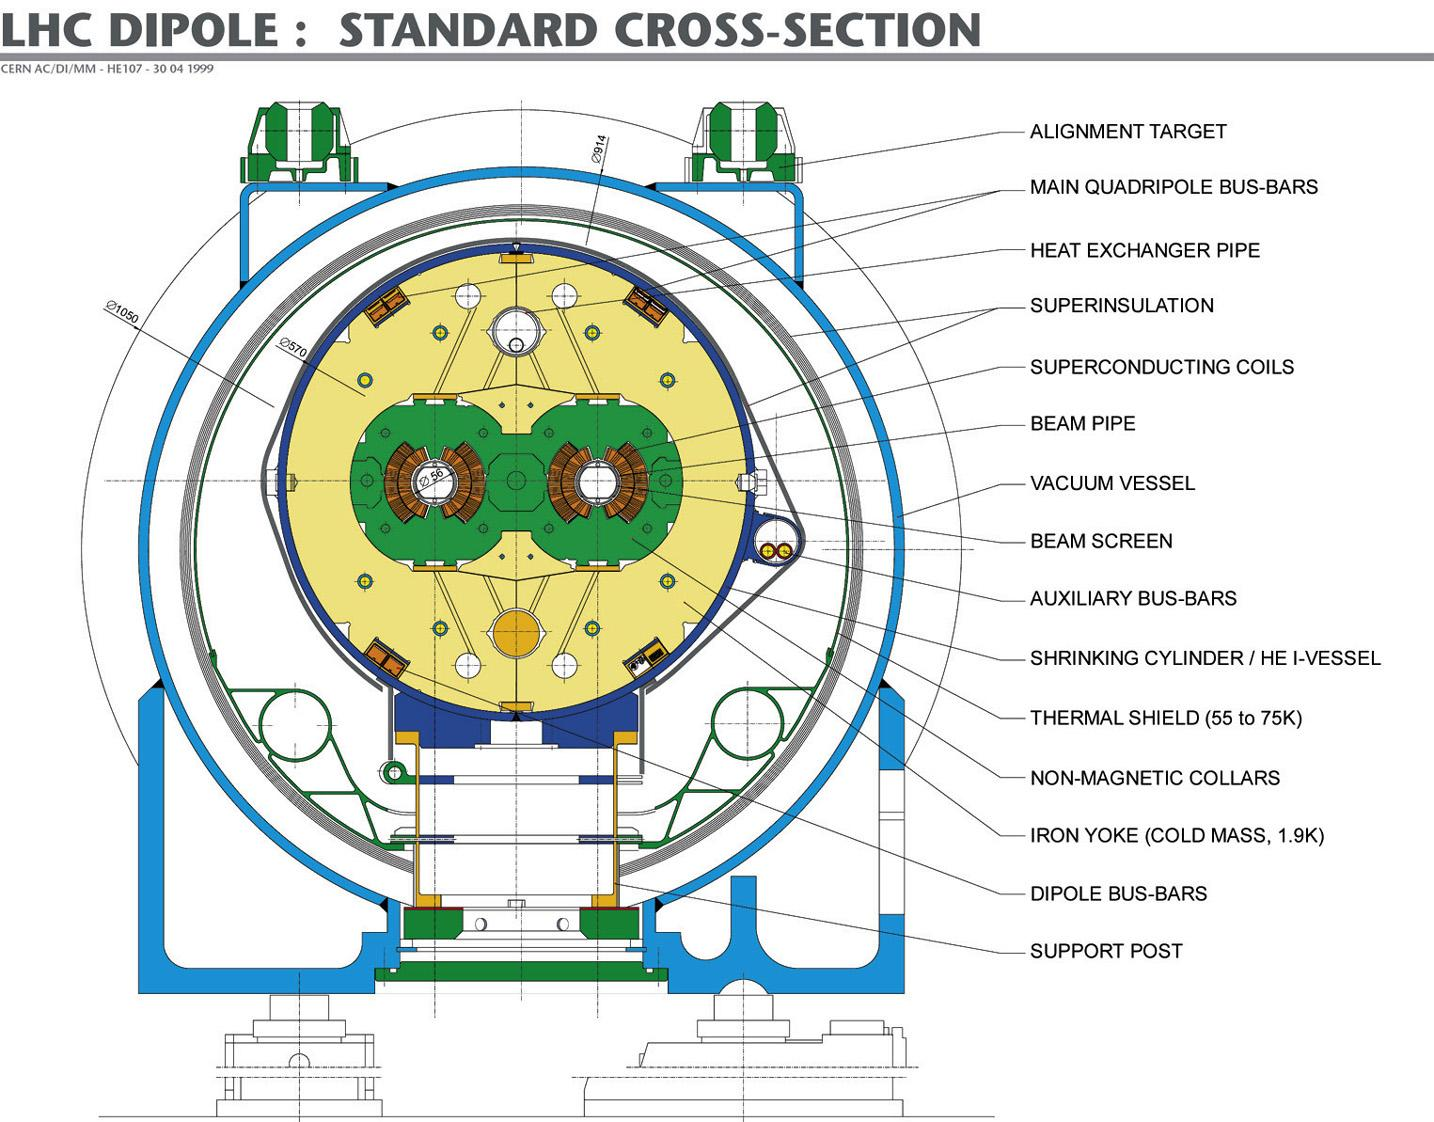
\includegraphics{figures/ch3-experiment/LHC_dipole_xsec}}
	}
	\caption{Two views of the LHC superconducting dipole magnet. The magnets are $15~\mbox{m}$ long and have two bores, one for each of the counter-rotating beams.}
	\label{fig:LHC-dipole-magnets}
\end{figure}

The acceleration is provided by two superconducting RF systems, one for each beam. The RF cavities are constructed from copper with a thin ($1-2~\micron$) layer of niobium, and operate at $4.5~\mbox{K}$. The single-cell cavities, each nominally providing $2~\mbox{MV}$, are arranged into cryomodules containing eight cells, for a total peak voltage of $16~\mbox{MV}$. A module consisting of two cells is shown in figure~\ref{fig:RF-module}. The RF frequency is $400~\mbox{MHz}$, giving an RF bucket length of $2.5~\mbox{ns}$, or $75~\mbox{cm}$. 

\begin{figure}[htbp]
	\centering
	\subfloat[ A prototype cryomodule containing two cavities.] {
		\resizebox{0.45\textwidth}{!}{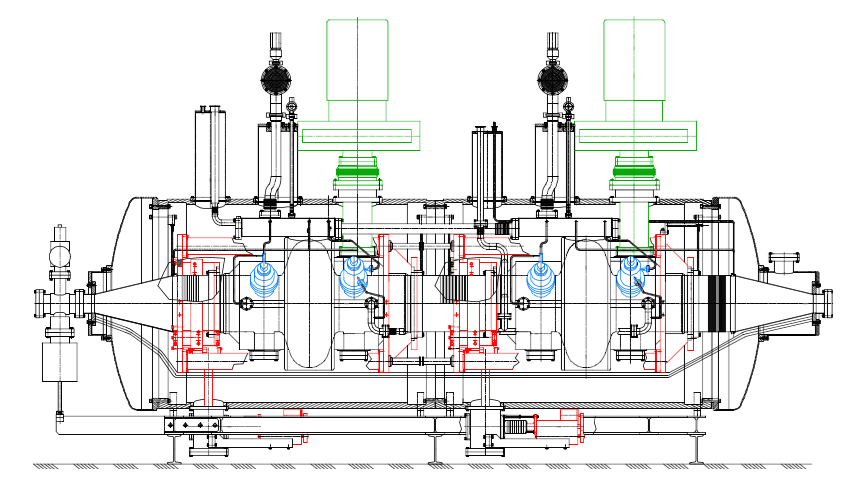
\includegraphics{figures/ch3-experiment/LHC_RF_cryomodule}}
	}
	\hfill
	\subfloat[ The RF cryomodules installed at IR4.] {
		\resizebox{0.45\textwidth}{!}{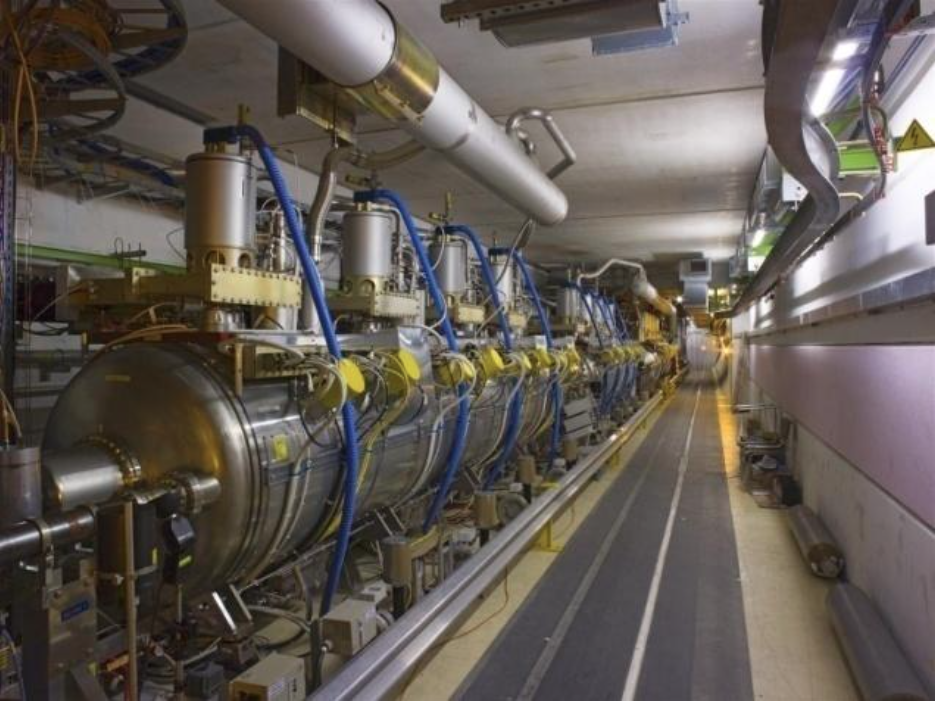
\includegraphics{figures/ch3-experiment/LHC_RF_IR4}}
	}
	\caption{The LHC RF cryomodules.}
	\label{fig:RF-module}
\end{figure}

At the collision points, the two beams converge in a single pipe for approximately $130~\mbox{m}$. A steering dipole directs the beams into collision, and a triplet of quadrupoles on each side of the interaction region focus the beam onto the interaction point, squeezing the beams in the transverse directions from a typical orbiting width of $\mathcal{O}(1~\mbox{mm})$ to a collision width of $\mathcal{O}(10~\micron)$. 


\subsection{Beam Parameters}
From the experiments' point of view, there are two main parameters to optimize in order to maximize sensitivity to new physics: the collision energy, $\sqrt{s}$, and the integrated luminosity, $\int L dt$. The collision energy is limited to $\sqrt{s}=14~\mbox{TeV}$ by the bending power of the dipole magnets, which have a nominal field strength of $8.33~\mbox{T}$; however, due to the faulty splice design mentioned above, the energy was limited to $\sqrt{s}=7-8~\mbox{TeV}$ in Run I. 

The optimization of luminosity is somewhat more complicated.  The instantaneous luminosity of the colliding beams is given by:
\begin{equation}\label{eqn:lumi}
	L = \frac{n_b f_r N_1 N_2 \gamma_b}{4\pi \epsilon_n \beta_{*}} F(\alpha),
\end{equation}
where $n_b$ is the number of colliding bunch pairs, $f_r=11245.5~\mbox{Hz}$ is the LHC revolution frequency, $N_{1,2}$ are the number of proton in the two beams, $\gamma_b$ is the relativistic gamma factor, $\epsilon_n$ is the normalized emittance, $\beta_{*}$ is the beta function at the collision point, and $F(\alpha)$ is the reduction in luminosity due to a nonzero beam crossing half-angle of $\alpha$. 

% TO DO: beta* formula?

In general, a higher total integrated luminosity, $L{\mathrm{int}}=\int L dt$, is desired. This depends on a number of factors:

\begin{itemize}
	\item The instantaneous luminosity per bunch, $L_b=\frac{f_r N_1 N_2}{4\pi\epsilon_n \beta_{*}}$. A higher $L_b$ increases the number of simultaneous collisions per bunch crossing (\emph{pileup}), $\mu=L_b/\sigma_{\mathrm{inel}}$, which degrades the performance of the experiments. 
	% Removed for now. According to Frank Zimmerman's slides, no beam-beam limit was found in MDs! 
	% From the accelerator's point of view, the number of protons per bunch, $N_{1,2}$, and the transverse emittance are limited by non-linear beam-beam effects~\cite{Papotti:2014vb}. Typical values during 2012 were $N_{1,2}=1.65\times 10^{11}$ and $\epsilon_n=2.5~\micron$, giving pileup values at the start of a fill of around 30, with tails up to $\sim$40. 

	\item The number of bunches in the LHC, $n_b$. During Run I, the LHC was filled with 1380 bunches with $50~\mbox{ns}$ spacing between bunches, as opposed to the nominal 2808 bunches with $25~\mbox{ns}$ spacing. The advantages of $50~\mbox{ns}$ spacing include less days needed for electron-cloud scrubbing, smalled transverse emittances, and a smaller crossing angle~\cite{Papotti:2014vb}. The primary disadvantage is a higher pileup for the experiments. 

	\item The crossing angle, $\alpha$. A nonzero crossing angle is required to prevent \emph{parasitic collisions} between bunches adjacent to the nominal collision point. For bunches spaced by $25~\mbox{ns}$, there are 34 unwanted parasitic collision points inside the common beam pipe at each interaction region. The reduction in luminosity is:

	\begin{equation}
		F(\alpha)=\frac{1}{\sqrt{1+\left(\frac{2\alpha \sigma_z}{2\sigma^*}\right)}},
	\end{equation}
	
	where $\sigma_z$ is the RMS bunch length and $\sigma^{*}$ is the transverse beam width at the collision point. During normal 2012 running conditions, the crossing half-angle was $\alpha=145~\mu\mbox{rad}$, and the luminosity reduction factor was about $18\%$. 

	\item The fill schedule of the LHC. The instantaneous luminosity of the LHC decreases over time. The dominant loss of luminosity is due to the loss of protons from the collisions themselves, with a typical decay constant of $\tau_{\mathrm{nuclear},1/e}=29~\mbox{h}$. Including other sources of loss such as intra-bunch scattering, scattering from collisions with gas in the beam pipe, beam-beam effects, and RF noise, the typical luminosity lifetime is $\tau_L=14.9~\mbox{h}$. 

	The the fill schedule can be optimized to maximize the luminosity based on $\tau_L$ and the average turnaround time, $T_{\mathrm{turnaround}}$. This can be quantified using the \emph{H{\"u}bner} factor, $\mathrm{HF}_{\mathrm{peak}}$, defined as the ratio of the delivered integrated luminosity to the hypothetical integrated luminosity with $\tau_L=\infty$ and $T_{\mathrm{turnaround}}=0$. In 2011, this was typically in the range $15\%$--$20\%$.
\end{itemize}

The delivered luminosity in 2011 and 2012 will be discussed later in section~\ref{sec:luminosity-measurement}.


\section{The ATLAS Experiment}\label{sec:the-atlas-experiment}

The ATLAS detector is a large, cylindrical collider detector located at IR1 on the LHC ring (figure~\ref{fig:LHC-IPs}). The detector measures the energy and momenta of charged and colored particles produced in the collisions provided by the LHC. It consists of several subsystems occupying a cylinder with a diameter of $25~\mbox{m}$ and a length of $46~\mbox{m}$, with a combined weight of approximately 7,000 tons. Closest to the interaction region, the inner detector performs momenta measurements of charged particles by tracking their movement through a solenoidal magnetic field (section~\ref{sec:inner-detector}). Past the inner detector solenoid magnet, electromagnetic and hadronic calorimeters measure the energy of electrons, photons, and hadrons. Finally, the muon spectrometer provides additional tracking and particle identification for muons in large toroidal magnetic field. 

This section describes the design of the magnets, inner detector, calorimeters, and muon spectrometer. The identification of objects and the associated performance are described in section~\ref{sec:object-reconstruction}. 

\subsection{Coordinate System}\label{sec:ATLAS-coordinate-system}

The ATLAS detector uses a right-handed coordinate system, with $\hat{x}$ pointing from the interaction point towards the center of the LHC ring, $\hat{y}$ pointing up, and $\hat{z}$ pointing along the ring towards IR2. Due to the symmetry of the detector, cylindrical coordinates ($r,\theta,\phi$) are often used, with $r$ the transverse distance from the beam line, $\theta$ the polar angle from the beamline, and $\phi$ the azimuthal angle in the $x$-$y$ plane. The polar angle can also be expressed in term of the pseudorapidity, $\eta = -\log \tan \frac{\theta}{2}$, which is useful for describing the geometry of particles in part because difference in pseudorapidity, $\Delta\eta$, are invariant under longitudinal Lorentz boost along $\hat{z}$. For massless particles, the pseudorapidity is equal to the rapidity, $y=\frac12 \log \frac{E+p_z}{E-p_z}$. 

\subsection{Magnets}\label{sec:ATLAS-magnets}
ATLAS relies on four powerful superconducting magnets to bend the trajectories of charged particles, allowing the tracking detectors to provide measurements of their momenta. The solenoid provides a $2~\mbox{T}$ axial magnetic field in the volume of the inner detector, while the barrel and two endcap toroids provide a toroidal magnetic field ranging from $0.5$--$1~\mbox{T}$ for the muon spectrometer. The geometry of the magnets is shown in figure~\ref{figure:ATLAS-magnets-sketch}. Key parameters for the magnet system are shown in table~\ref{table:ATLAS-magnet-parameters}.

\begin{figure}[htbp]
	\centering
	\resizebox{0.6\textwidth}{!}{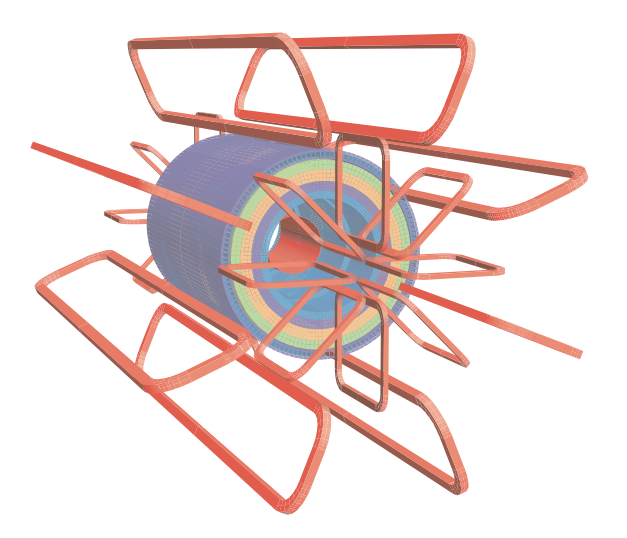
\includegraphics{figures/ch3-experiment/ATLAS_magnets_sketch}}
	\caption{The geometry of the magnet windings and tile calorimeter steel. The three toroids and solenoid are shown in red. The remaining colors show layers of the tile calorimeter with different magnetic properties and an outside return yoke.}
	\label{fig:ATLAS_magnets-sketch}
\end{figure}


\begin{table}[htbp]
	\centering
	\begin{tabular}{|l|l|c|c|c|c|}
		\hline
		\textbf{Property} & \textbf{Feature} & \textbf{Unit} & \textbf{Solenoid} & \textbf{Barrel toroid} & \textbf{End-cap toroids} \\
		\hline
		\textbf{Size} & Inner diameter & m & $2.46$ & $9.4$ & $1.65$ \\
		\hline
		 & Outer diameter & m & $2.56$ & $20.1$ & $10.7$ \\
		\hline
		 & Axial length & m & $5.8$ & $25.3$ & $5.0$ \\
		\hline
		 & Number of coils & & $1$ & $8$ & $2\times 8$ \\
		\hline
		\textbf{Mass} & Conductor & t & $3.8$ & $118$ & $2\times 20.5$ \\
		\hline
		 & Cold mass & t & $5.4$ & $370$ & $2\times 140$ \\
		\hline
		 & Total assembly & t & $5.7$ & $830$ & $2\times 239$ \\
		\hline
		\textbf{Coils} & Turns per coil & & $1154$ & $120$ & $116$ \\
		\hline
		 & Nominal current & kA & $7.73$ & $20.5$ & $20.5$ \\
		\hline
		 & Magnet stored energy & GJ & $0.04$ & $1.08$ & $2\times 0.25$ \\
		\hline
		 & Peak field in the windings & T & $2.6$ & $3.9$ & $4.1$ \\
		\hline
		 & Field range in the bore & T & $0.9$-$2.0$ & $0.2$-$2.5$ & $0.2$-$3.5$ \\
		\hline
		\textbf{Conductor} & Overall size & mm$^2$ & $30\times 4.25$ & $57\times12$ & $41\times 12$ \\
		\hline
		 & Ratio Al:Cu:NbTi & & $15.6:0.9:1$ & $28:1.3:1$ & $19:1.3:1$ \\
		\hline
		 & Number of strands (NbTi) & & $12$ & $38$-$40$ & $40$ \\
		\hline
		 & Strand diameter (NbTi) & mm & $1.22$ & $1.3$ & $1.3$ \\
		\hline
		 & Critical current (at $5~\mbox{T}$ and $4.2~\mbox{K}$) & kA & $20.4$ & $58$ & $60$ \\
		\hline
		 & Operating/critical current ratio at $4.5~\mbox{K}$ & \% & $20$ & $30$ & $30$ \\
		\hline
		 & Residual resistivity ratio (RRR) for Al & & $>500$ & $>800$ & $>800$ \\
		\hline
		 & Temperature margin & K & $2.7$ & $1.9$ & $1.9$ \\
		\hline
		 & Number of units $\times$ length & m & $4\times 2290$ & $8\times 4 \times 1730$ & $2\times8\times2\times800$ \\
		\hline
		 & Total length (produced) & km & $10$ & $56$ & $2\times13$ \\
		\hline
		\textbf{Heat load} & At $4.5~\mbox{K}$ & W & $130$ & $990$ & $330$ \\
		\hline
		 & At $60$-$80~\mbox{K}$ & kW & $0.5$ & $7.4$ & $1.7$ \\
		\hline
		 & Liquid helium mass flow & g/s & $7$ & $410$ & $280$ \\
		\hline
	\end{tabular}
	\caption{Main parameters of the ATLAS magnet system. From~\cite{TheATLASCollaboration:2008fg}.}
	\label{table:ATLAS-magnet-parameters}
\end{table}




\subsubsection{Solenoid}\label{sec:ATLAS-magnets-solenoid}

The central solenoid is shown in figure~\ref{fig:solenoid}. The solenoid consists of a single coil with 1154 windings made of high strength Al-stabilized NbTi conductor. The coil has an inner radius of $2.46~\mbox{m}$, an outer radius of $2.56~\mbox{m}$, and a length of $5.8~\mbox{m}$. With a nominal current of $7.73~\mbox{kA}$, the magnetic field is $1.998~\mbox{T}$ at the center of the solenoid, falling to $1.8~\mbox{T}$ at $z=1.7~\mbox{m}$ and $0.9~\mbox{T}$ the end of the inner detector cavity. The magnetic flux is returned via the steel in the hadronic calorimeter and its support structures. Liquid helium is used to cool the superconducting coil to an operating temperature of $4.5~\mbox{K}$. At nominal current, the stored energy is $40~\mbox{MJ}$. 

The magnetic field at $z=0$ is shown in figure~\ref{fig:ATLAS-solenoid-Bfield}.

\begin{figure}[htbp]
	\centering
	\resizebox{0.6\textwidth}{!}{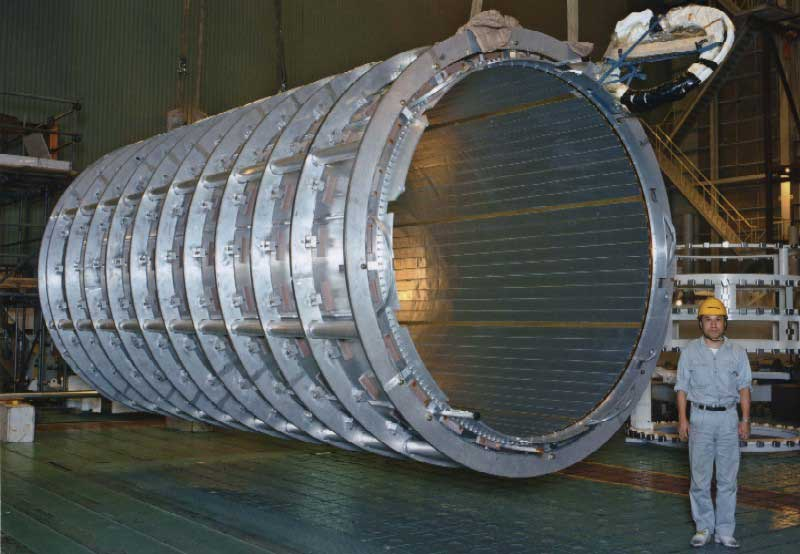
\includegraphics{figures/ch3-experiment/ATLAS_solenoid_2}}
	\caption{The central solenoid in the factory after completion of the coil winding~\cite{TheATLASCollaboration:2008fg}.}
	\label{fig:solenoid}
\end{figure}

\begin{figure}[htbp]
	\centering
	\resizebox{0.6\textwidth}{!}{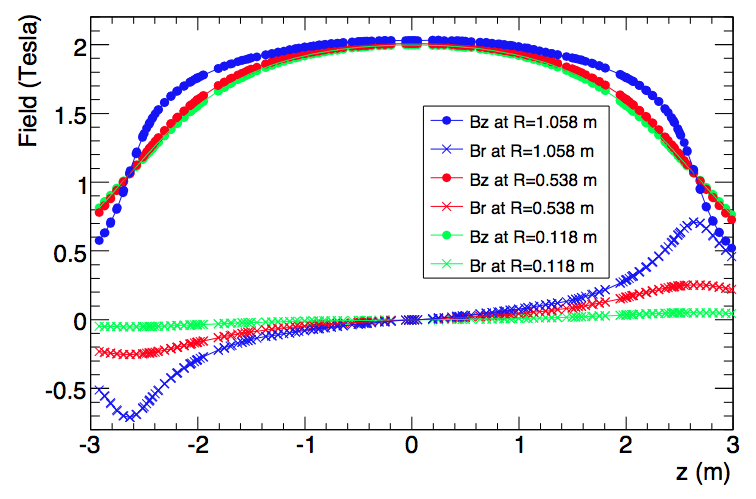
\includegraphics{figures/ch3-experiment/ATLAS_solenoid_Bfield}}
	\caption{The solenoid magnetic field in the radial ($B_r$) and longitudinal ($B_z$) directions, shown for $z=0$ and $\phi=20\pi/16$ at different values of $r$. The field determined from a fit of the field model to measurements using an array of Hall probes~\cite{Aleksa:2008br}.}
	\label{fig:ATLAS-solenoid-Bfield}
\end{figure}



\subsubsection{Toroid}\label{sec:ATLAS-magnets-toroid}

The magnetic field for the muon spectrometer is provided by three large toroid magnets, each with eight superconducting coils. The magnets are shown in figure~\ref{fig:ATLAS-toroids}. The barrel toroid measures $25.3~\mbox{m}$ in length, with inner and outer diameters of $9.4~\mbox{m}$ and $20.1~\mbox{m}$, respectively. The two end-cap toroids are $5.0~\mbox{m}$ in length, with inner and outer diameters of $1.65~\mbox{m}$ and $10.7~\mbox{m}$, respectively. Both types of toroid contain eight coils, with 120 windings each in the barrel and 116 windings each in the end-caps. The endcap coils are rotated by $22.5^{\circ}$ from the barrel coils to optimize the bending power in the overlap region between the magnets. Like the solenoid, the conductor is Al-stabilized NbTi, operated at $4.5~\mbox{K}$. The nominal current is $20.5~\mbox{kA}$, producing a magnetic field that varies from $0.15~\mbox{T}$ to $2.5~\mbox{T}$ in the barrel region, and $0.2~\mbox{T}$ to $3.5~\mbox{T}$ in the end-caps. The bending power of the toroid is shown as a function of $\eta$ in figure~\ref{fig:toroid-bending-power}. The total stored energy at nominal current is $1.58~\mbox{GJ}$. 

The field integral of the toroid is shown as a function of $\eta$ in figure~\ref{fig:ATLAS-toroid-Bintegral}. The field integral drops at the boundary between the barrel and end-caps, where the fields from the two magnets partially cancel. 

\begin{figure}[htbp]
	\centering
	\subfloat[ Barrel toroid.] {
		\resizebox{0.45\textwidth}{!}{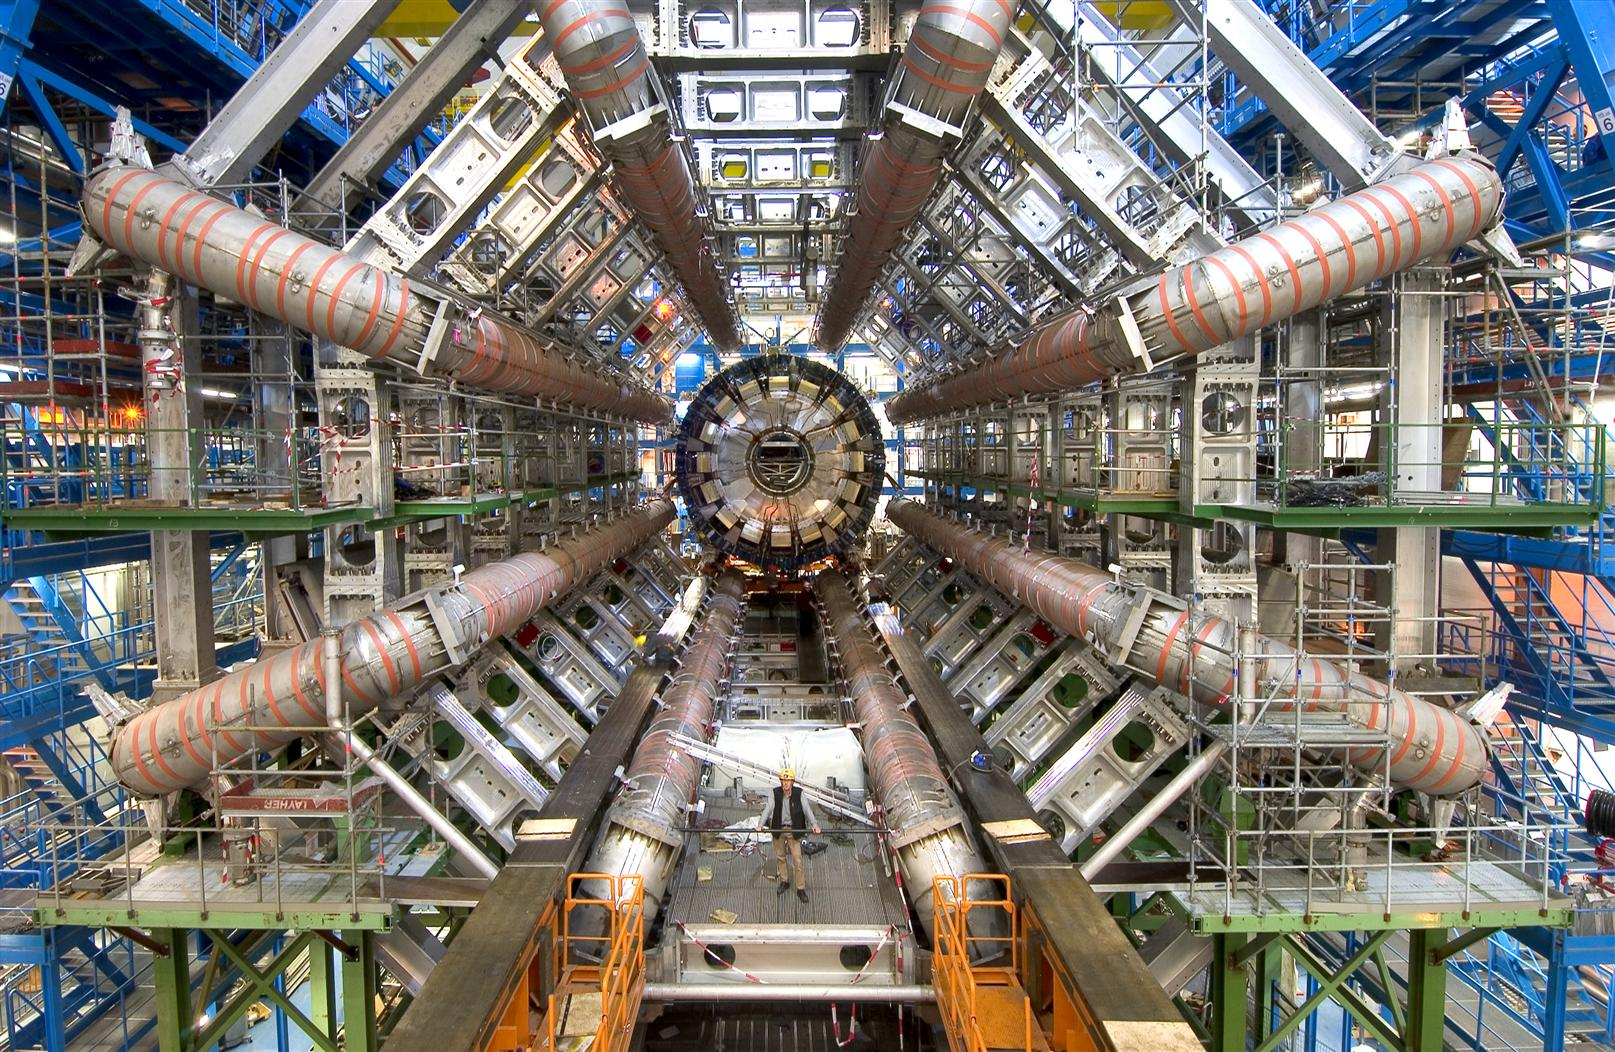
\includegraphics{figures/ch3-experiment/ATLAS_toroid}}
	}
	\hfill
	\subfloat[ End-cap toroid, inserted into the barrel toroid.] {
		\resizebox{0.45\textwidth}{!}{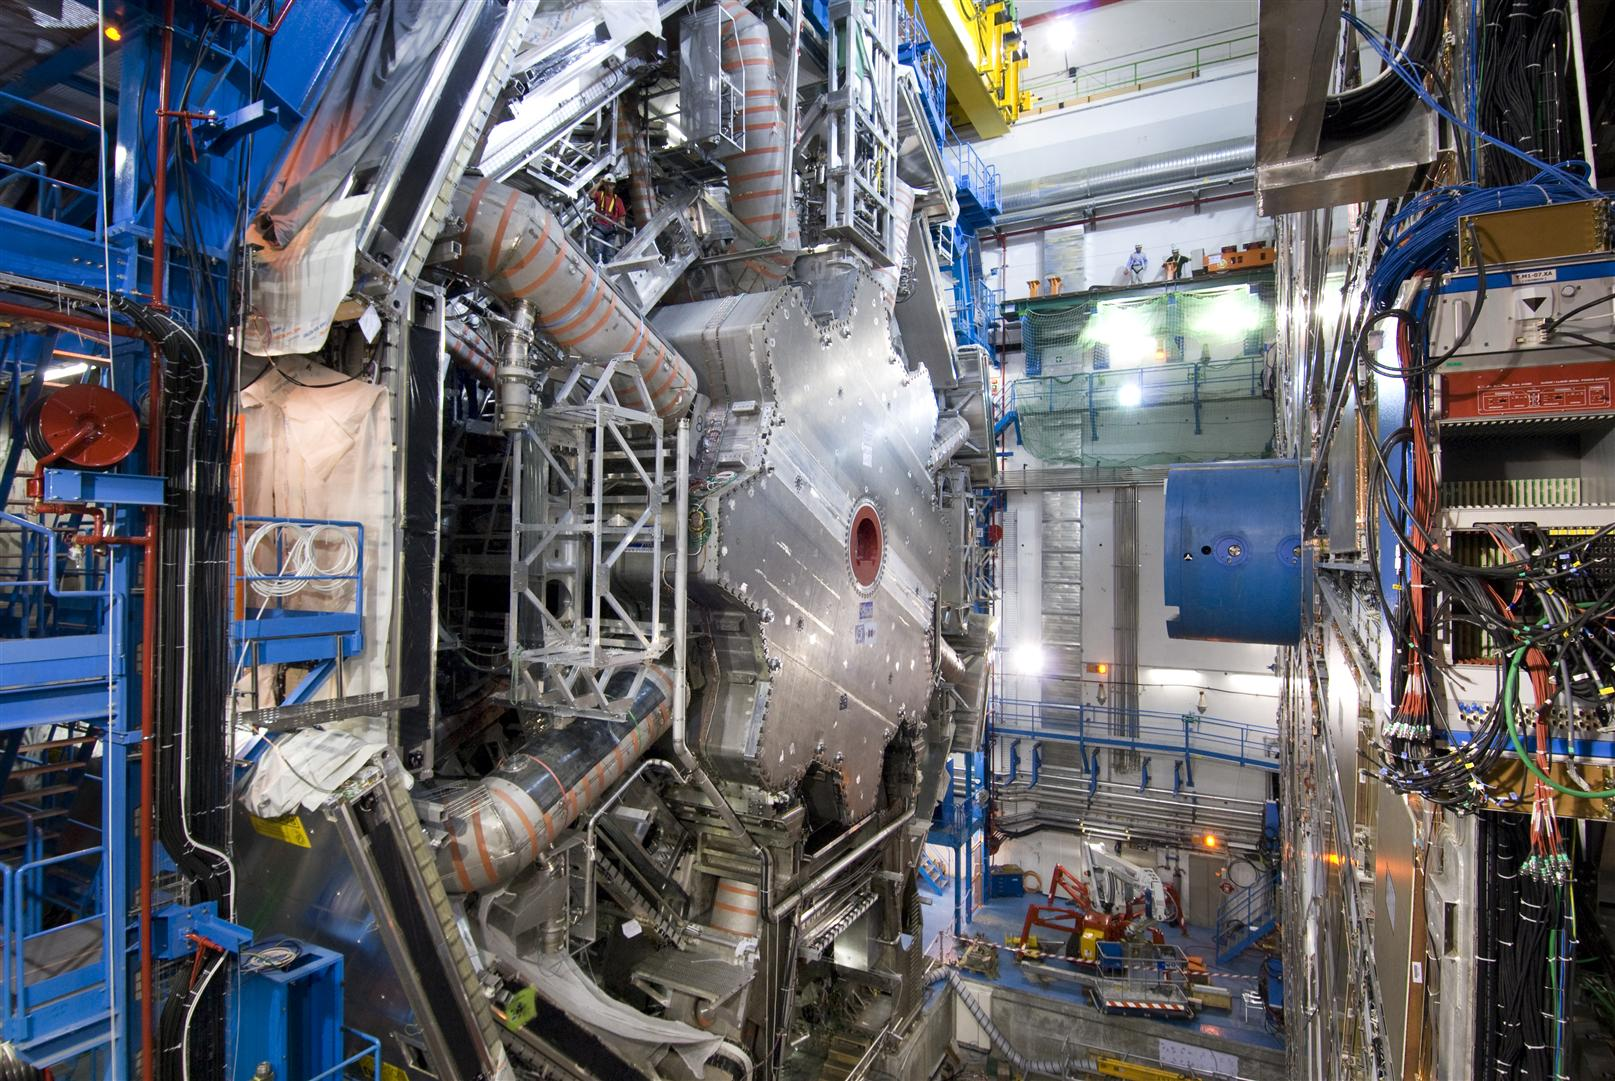
\includegraphics{figures/ch3-experiment/ATLAS_toroid_endcap_inserted2}}
	}
	\caption{Images of the barrel and end-cap toroid magnets during installation.}
	\label{fig:ATLAS-toroids}
\end{figure}

\begin{figure}[htbp]
	\centering
	\resizebox{0.6\textwidth}{!}{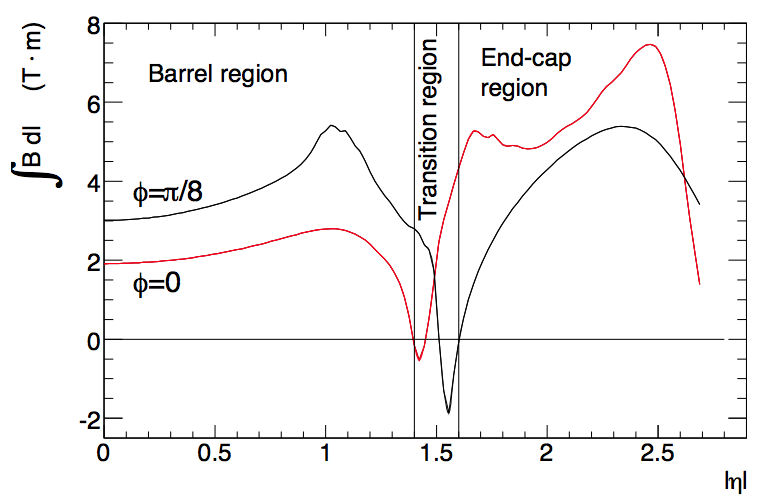
\includegraphics{figures/ch3-experiment/ATLAS_toroid_Bintegral}}
	\caption{The predicted toroid magnetic field integral as a function of $|\eta|$. The paths are for infinite momentum muons, i.e. straight lines, from the innermost to the outermost MDT layer (section~\ref{sec:muon-spectrometer}).}
	\label{fig:ATLAS-toroid-Bintegral}
\end{figure}



\subsection{Inner Detector}\label{sec:ATLAS-inner-detector}

The inner detector performs tracking charged particles traversing the $2~\mbox{T}$ solenoidal magnetic field in the region $|\eta|<2.5$. It also performs electron identification in the range $|\eta|<2.0$. It consists of three subdetectors occupying the volume closest to the interaction region, directly outside the beam pipe, as shown in figure~\ref{fig:ATLAS-ID}. Proceeding outwards from the interaction point, these are the pixel detector, the semiconductor tracker (SCT), and the transition radiation tracker (TRT). The pixel detector nominally provides three track measurements with high spatial resolution using silicon pixels. The SCT provides an additional four measurements using silicon strips. Finally, for particles with $|\eta|<2.0$, the TRT provides an average of 36 measurements per track using gaseous straw tubes, which aids the pattern recognition, improves the momentum resolution, and performs electron identification. The paths traversed by tracks through the barrel and end-cap layers are shown in figure~\ref{fig:ATLAS-ID-tracks}.

\begin{figure}[htbp]
	\centering
	\subfloat[ 3D model of the inner detector, showing the arrangement of the pixel detector, SCT, and TRT in the barrel and end-caps.] {
		\resizebox{0.45\textwidth}{!}{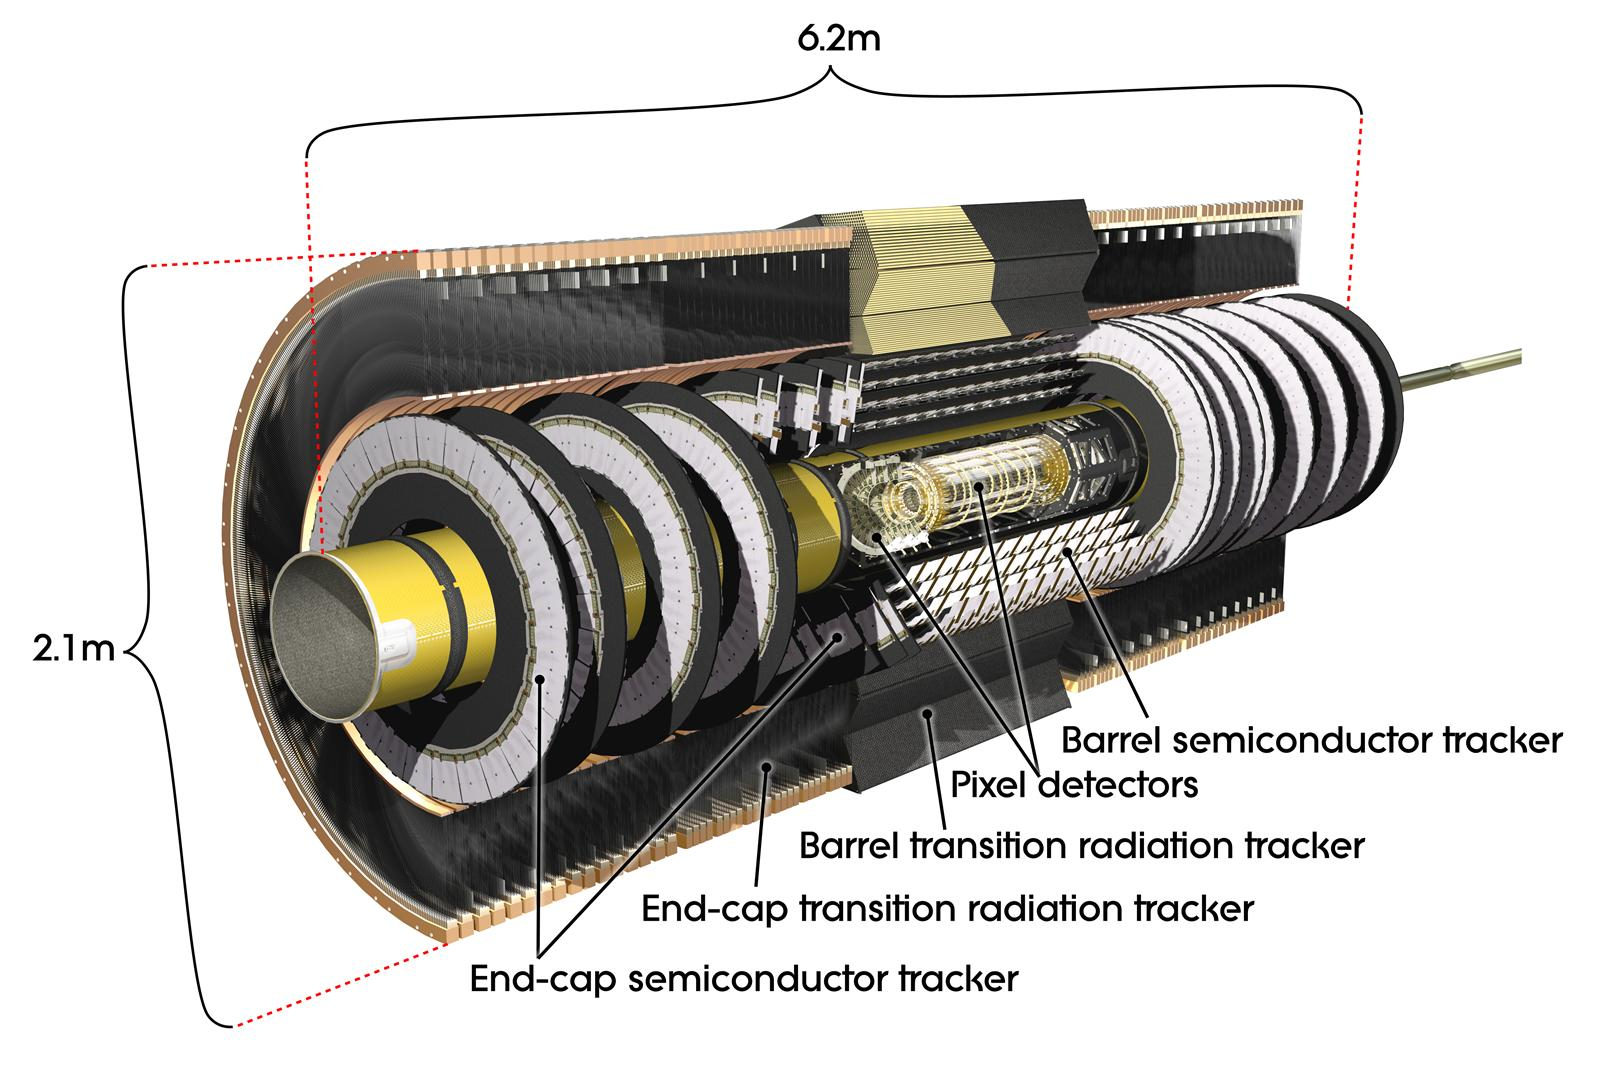
\includegraphics{figures/ch3-experiment/ATLAS_ID_sketch}}
	}
	\hfill
	\subfloat[ Layout of the inner detector in the $r-z$ plane.] {
		\resizebox{0.45\textwidth}{!}{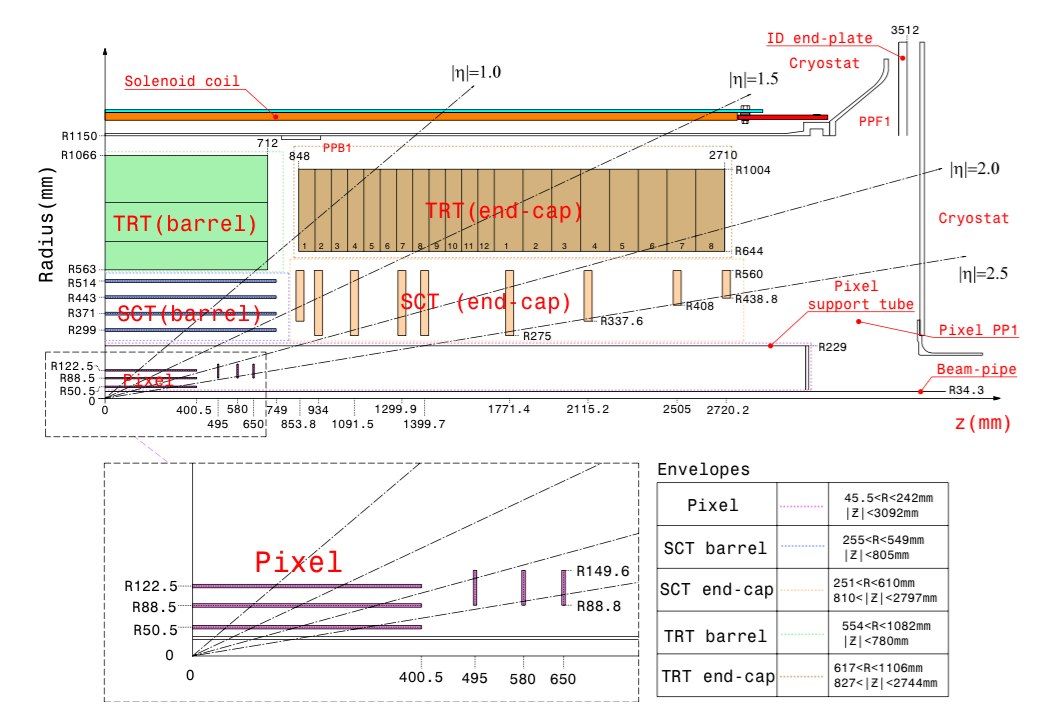
\includegraphics{figures/ch3-experiment/ATLAS_ID_layout_rz}}
	}
	\caption{Layout of the ATLAS inner detector.}
	\label{fig:ATLAS-ID}
\end{figure}

\begin{figure}[htbp]
	\centering
	\subfloat[ Trajectory of a $10 \GeV$ charged particle with $\eta=0.3$ traversing the barrel elements of the inner detector.] {
		\resizebox{0.45\textwidth}{!}{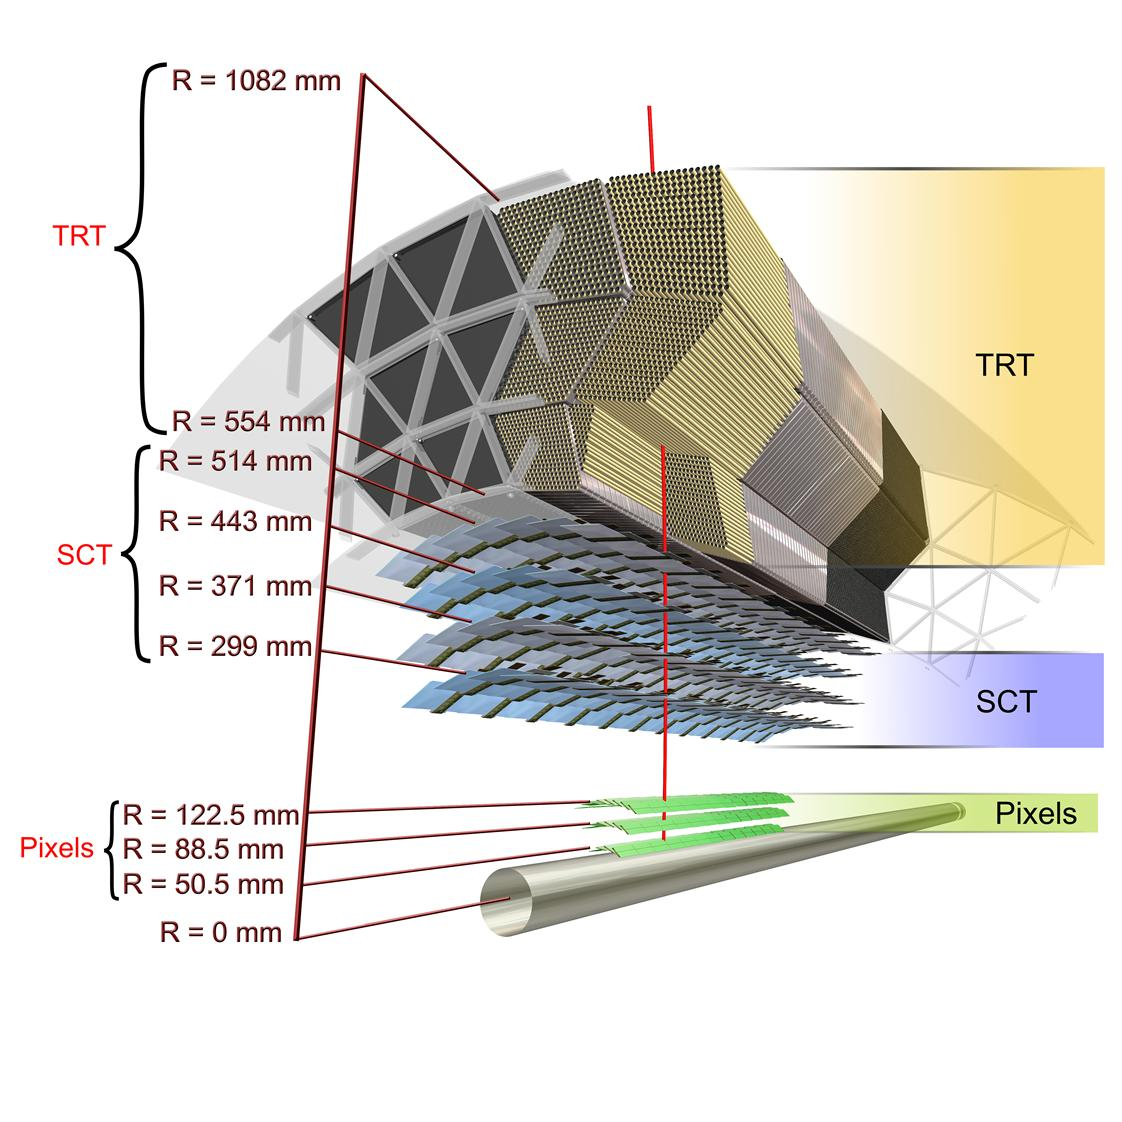
\includegraphics{figures/ch3-experiment/ATLAS_ID_track_barrel}}
	}
	\hfill
	\subfloat[ Trajectories of $10 \GeV$ charged particles with $\eta=1.4$ and $\eta=2.2$ traversing the barrel and end-cap elements of the inner detector.] {
		\resizebox{0.45\textwidth}{!}{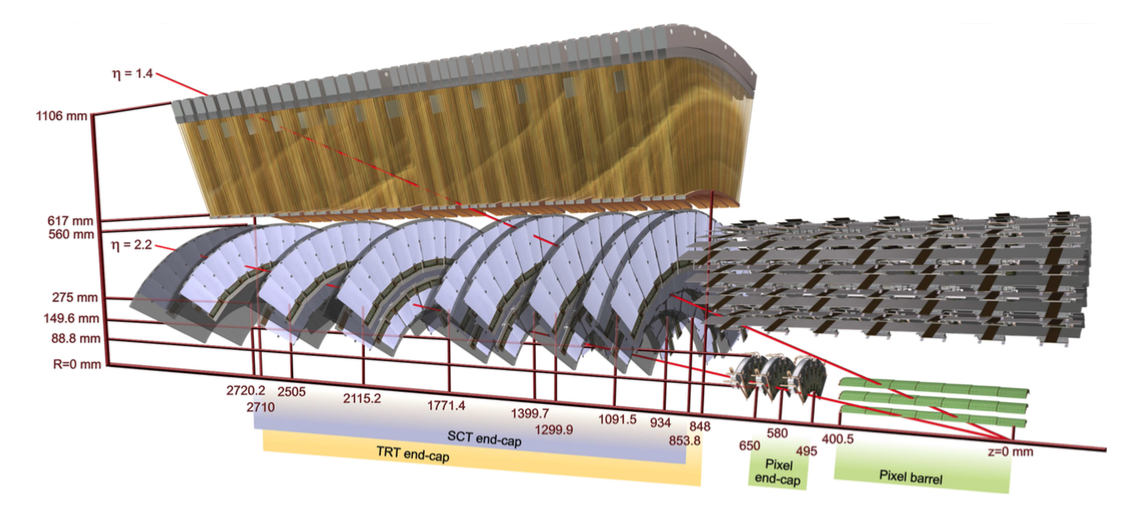
\includegraphics{figures/ch3-experiment/ATLAS_ID_track_endcap}}
	}
	\caption{Drawings of the inner detector sensors and structural elements traversed by $10 \GeV$ charged particles originating from the interaction point at various angles.}
	\label{fig:ATLAS-ID-tracks}
\end{figure}


\subsubsection{Pixel Detector}\label{sec:ATLAS-id-pixel-detector}

The pixel detector consists of 1744 identical pixel sensors, each measuring $19\times63~\mbox{mm}^2$ and containing $144\times 328=47232$ pixels, for a total of $80.4\times 10^6$ pixels. The size of the pixels is dictated by the front-end electronics: in 128 of the 144 columns, the pixels have a pitch of $50\times 400 \micron^2$, while the remaining 16 columns have a pitch of $50\times 600 \micron^2$. For space reasons, eight pairs of pixels in each column are ganged to a common readout, giving a total of 46080 readout channels per sensor.

 The sensors are $256~\micron$-thick detectors constructed from $n$-type wafers, with high dose positive ($p^+$) and negative ($n^+$) dose regions implanted on each side of a wafer. Initially, the asymmetric depletion region at the $p^+-n$ junction is operated in reverse bias with a voltage of $150~\mbox{V}$, and fills the sensor bulk volume, shown in figure~\ref{fig:ATLAS-pixel-normal}. The charge carriers generated by the passage of an ionizing particle through the bulk are collected at the $n^+$ side of the sensor, where the readout electronics are bump-bonded to the pixel. The nominal threshold for readout is about 3,500 electrons, which a minimally ionizing particle cross a pixel leaves a signal of about 20,000 electrons. However, over time, radiation damage induces type inversion in the bulk, after which the junction moves to the $n^+$ side of the sensor and the depletion zone grow from the pixel side, as shown in figure~\ref{fig:ATLAS-pixel-inverted}. The double-sided construction thus allows the pixel sensors to continue operating after type inversion.

The pixel sensors are assembled into pixel modules, shown in figure~\ref{fig:ATLAS-pixel-module}. Each modules contains 16 front-end electronics chips each with 2880 electronics channels. The front-ends are bump bonded to the pixel sensor elements. The other side of the pixel sensor tile is glued to a flexible polyimide printed circuit board (\emph{flex-hybrid}) that houses the module control chip.

The layout of the pixel detector is summarized in table~\ref{table:ATLAS-pixel-layout}.  The modules are assembled into staves in the barrel region, each with 13 pixel modules, and sectors in the end-caps, each with 6 pixel modules. The barrel layers consist of 22, 38, and 52 staves for layers 0, 1, and 2, respectively, while the end-caps each contain eight sectors. In the barrel, to provide complete coverage, the pixel staves overlap and are mounted with a tilt angle of $20^{\circ}$ between the normal to the module surface and $\hat{r}$, in the $\hat{\phi}$ direction. 

In the barrel, the pixels have an intrinsic accuracy of $10~\micron$ in the $R-\phi$ direction and $115~\micron$ in the $z$ direction, while in the end-caps, the intrinsic accuracy is $10~\micron$ in the $R-\phi$ direction and $115~\micron$ in the $R$ direction.

\begin{table}[htbp]
	\centering
	\begin{tabular}{|l|c|c|c|c|}
		\hline
		\textbf{Barrel} & \textbf{Radius (mm)} & \textbf{Modules} & \textbf{Pixels} \\
		\hline
		Layer-0 & $50.5$ & $22$ & $286$ & $13.2\times 10^6$ \\
		Layer-1 & $88.5$ & $38$ & $494$ & $22.8\times 10^6$ \\
		Layer-2 & $112.5$ & $52$ & $676$ & $31.2\times 10^6$ \\
		\hline
		\textbf{End-cap (one side)} & $z$ \textbf{(mm)} & \textbf{Sectors} & \textbf{Modules} & \textbf{Pixels} \\
		\hline
		Disk 1 & $495$ & $8$ & $48$ & $2.2\times 10^6$ \\
		Disk 2 & $495$ & $8$ & $48$ & $2.2\times 10^6$ \\
		Disk 3 & $495$ & $8$ & $48$ & $2.2\times 10^6$ \\
		\hline
		\textbf{Barrel and both end-caps} & & $1744$ & $80.4\times 10^6$ \\
		\hline
	\end{tabular}
	\caption{Parameters of the pixel detector, from~\cite{TheATLASCollaboration:2008fg}.}
	\label{table:ATLAS-pixel-layout}
\end{table}

\subsubsection{SCT}\label{sec:ATLAS-id-sct}

The SCT consists of 15912 sensors using single-sided, p-in-n type silicon strips. The use of single-sided strips lowers both the cost and the number of readout channels of the detector, which covers significantly more area than the pixel detector ($61.1~\mbox{m}^2$ versus $2.3~\mbox{m}^2$). In the barrel, the strips have a pitch of $80~\micron$ and a length of $12~\cm$. In the endcaps, the sensors are trapezoidal with radially arranged strips, with a mean strip pitch of $80~\micron$ and a length of $12~\cm$. Each sensor has 768 active strips. Like the pixel sensors, the operating voltage will be $\sim150~\mbox{V}$ initially, and will increase to $250$-$350~\mbox{V}$ after several years of irradiation, depending on the location of the sensor. 

The SCT modules are shown in figure~\ref{fig:ATLAS-SCT-modules}.The 2112 barrel modules contain four sensors, while the 1976 end-cap modules contain two sensors. In both cases, the sensors are glued to a $380~\micron$-thick thermal pyrolitic graphite (TPG) base-board. The sensors are assembled in two layers with a rotation of $\pm 20~\mbox{mrad}$ about the center of the sensors. The stereo angle between the two sensors allows for a measurement of the position along the length of the sensors. 

% Arrangement into barrel layers and end-caps

The intrinsic accuracy of the SCT sensors is $17~\micron$ along the strip pitch, corresponding to the $R-\phi$ direction. Along the length of the strips, the stereo angle allows for position measurement with an accuracy of $580~\micron$, corresponding to the $z$ direction in the barrel and the $R$ direction in the end-caps.

\begin{table}[htbp]
	\centering
	\begin{tabular}{|l|c|c|c|c|}
		\hline
		\textbf{Barrel cylinder layer} & \textbf{Radius (mm)} & \textbf{Full length (mm)} & \textbf{Module tilt angle} & \textbf{Number of modules} \\
		\hline
		3 & $299$ & $1498$ & $11.00^{\circ}$ & $384$ \\
		4 & $371$ & & $11.00^{\circ}$ & $480$ \\
		5 & $443$ & & $11.25^{\circ}$ & $576$ \\
		6 & $514$ & & $11.25^{\circ}$ & $672$ \\
		\hline
	\end{tabular}
	\caption{The dimensions and arrangement of modules in the four SCT layers. The tilt angle is between the normal to the module surface and $\hat{r}$, in the $\hat{\phi}$ direction.}
	\label{fig:ATLAS-SCT-layout}
\end{table}

\subsubsection{TRT}\label{sec:ATLAS-id-trt}

The TRT detector elements are polyimide drift (straw) tubes. The straws are arranged such that charged particles with $\pt > 500~\MeV$ and $|\eta|<2.0$ traverse at least 36 straws, except in the barrel/end-cap transition region where particles traverse as few as 22 straws. The straws are interleaved with polypropylene fibers in the barrel and polypropylene foils in the end-caps to provide transition radiation; electrons with $\pt>2.0~\GeV$ typically leave $7$-$10$ high-threshold hits. The intrinsic resolution of the straws is $130~\micron$ in the transverse direction.

The straws measure $4~\mm$ in diameter and $144~\cm$ ($37~\cm$) in length in the barrel (end-caps). The straw walls consist of two $35~\micron$ films bonded back-to-back. The base film material is a $25~\micron$ thick layer of polyamide, which is coated on the exterior side with a $0.2~\micron$ thick layer of Al and a $5$-$6~\micron$ thick protective layer of graphite-polyamide. The other side of the film is coated with a $5$-$6~\micron$ thick layer of polyurethane, which is used to heat-seal the two film layers together. The anodes of the detectors are tungsten wires running down the axis of the tubes, with $31~\micron$ diameter and plated with $0.5$-$0.7~\micron$ of gold. The wires are supported at the end of the straw by an end plug, where they connect to the front-end electronics. At the middle of the straw, the wires are supported by a plastic insert, and are also split electrically by a fused glass capillary to reduce occupancy. The active length of each half of the wire is $71.2~\cm$, with a $2~\cm$ inefficient length at the middle. The signal attenuation length is $\sim 4~\mbox{m}$, and the signal propagation time is $\sim 4 \mbox{ns}/\mbox{m}$. The straws are filled with a mixture of 70\% Xe, 27\% CO$_2$, and $3\%$ O$_2$. With a cathode voltage of $-1530~\mbox{V}$, the gain in the straws is $2.5\times 10^4$.

The layout of the straws in the barrel and end-caps is summarized in table~\ref{table:ATLAS-TRT-layout}. In the barrel, the straws are arranged into three layers of modules as shown in figure~\ref{fig:barrel-modules}, with different dimensions and straw counts depending on the layer. The straws are interleaves with transition radiation material, polypropylene fibers measuring $19~\micron$ in diameter. The module shell is made from $400~\micron$ thick carbon fiber, and serve not only as a support structure, but also as a gas manifold for CO$_2$, which prevents high-voltage discharges, flushes any Xe leaking from the straws, and conducts heat away from the straws.  

The endcaps consist of 160 layers of 768 straws, arranged radially into 20 wheels with 8 layers each. The inner 12 wheels (type-A) are spaced $8~\mm$ in $z$, while the outer 8 wheels (type-B) are spaced by $15~\mm$. Each successive layer in a wheel is separated by a $15~\micron$ thick polypropylene radiator foil, and is rotated by $3/8$ of the azimuthal straw spacing to optimize the uniformity of the number of straw crossed.


\begin{table}[htbp]
	\centering
	\begin{tabular}{|l|c|c|c|c|c|}
		\hline
		 & $z$ (mm) & $R$ (mm) & Modules & Layers & Straws/Module \\
		 \hline
		 \textbf{Barrel (both sides)} & $\mathbf{0\mhyphen780}$ & $\mathbf{554\mhyphen1082}$ & $\mathbf{96}$ & $\mathbf{73}$ & $\mathbf{52544}$ \\
		 Type-1 module (inner) & $400\mhyphen712.1$ & $563\mhyphen624$ & \multirow{2}{*}{$32$} & $9$ & \multirow{2}{*}{$329$} \\
		 Type-1 module (outer) & $7.5\mhyphen712.1$ & $625\mhyphen 694$ & & $10$ & \\
		 Type-2 module & $7.5\mhyphen 712.1$ & $697\mhyphen860$ & $32$ & $24$ & $520$ \\
		 Type-3 module & $7.5\mhyphen 712.1$ & $863\mhyphen 1066$ & $32$ & $30$ & $793$ \\
		 \hline
		 \textbf{End-cap (one side)} & $\mathbf{827\mhyphen 2744}$ & $\mathbf{615\mhyphen1106}$ & $\mathbf{20}$ & $\mathbf{160}$ & $\mathbf{122880}$ \\
		 Type-A wheels & $848\mhyphen1705$ & $644\mhyphen1004$ & $12$ & $8$ & $6144$ \\
		 Type-B wheels & $1740\mhyphen2710$ & $644\mhyphen1004$ & $8$ & $8$ & $6144$ \\
		 \hline
	\end{tabular}
	\caption{Layout and straw counts of the TRT barrel modules and end-cap wheels. The totals for the barrel and end-caps, shown in bold, include services and electronics.}	
	\label{table:ATLAS-TRT-layout}
\end{table}


\subsection{Calorimetry}\label{sec:ATLAS-calorimeters}
The calorimeter system occupies the volume directly exterior to the solenoid magnet, and measures the energy of electrons, photon, and hadrons up to a pseudorapidity of $|\eta|=4.9$. The arrangement of the calorimeters is shown in figure~\ref{fig:ATLAS-calorimeters}. The system consists of a number of independent sampling calorimeters. The electromagnetic calorimeter measures the energy of electrons and photons using lead and liquid argon (LAr) to measure the energy of electrons and photons. The hadronic calorimeter measures the energy of hadrons using steel and scintillator tiles in the barrel and copper and LAr in the end-caps. Finally, electromagnetic and hadronic calorimetry is performed in the forward region using copper-LAr and tungsten-LAr technology. Besides performing energy measurements, the calorimeters providing containment electrons, photons, and hadrons, which effectively provides shielding for the muon spectrometer~\ref{sec:ATLAS-muon-spectrometer}. 

\begin{figure}[htbp]
	\centering
	\resizebox{0.6\textwidth}{!}{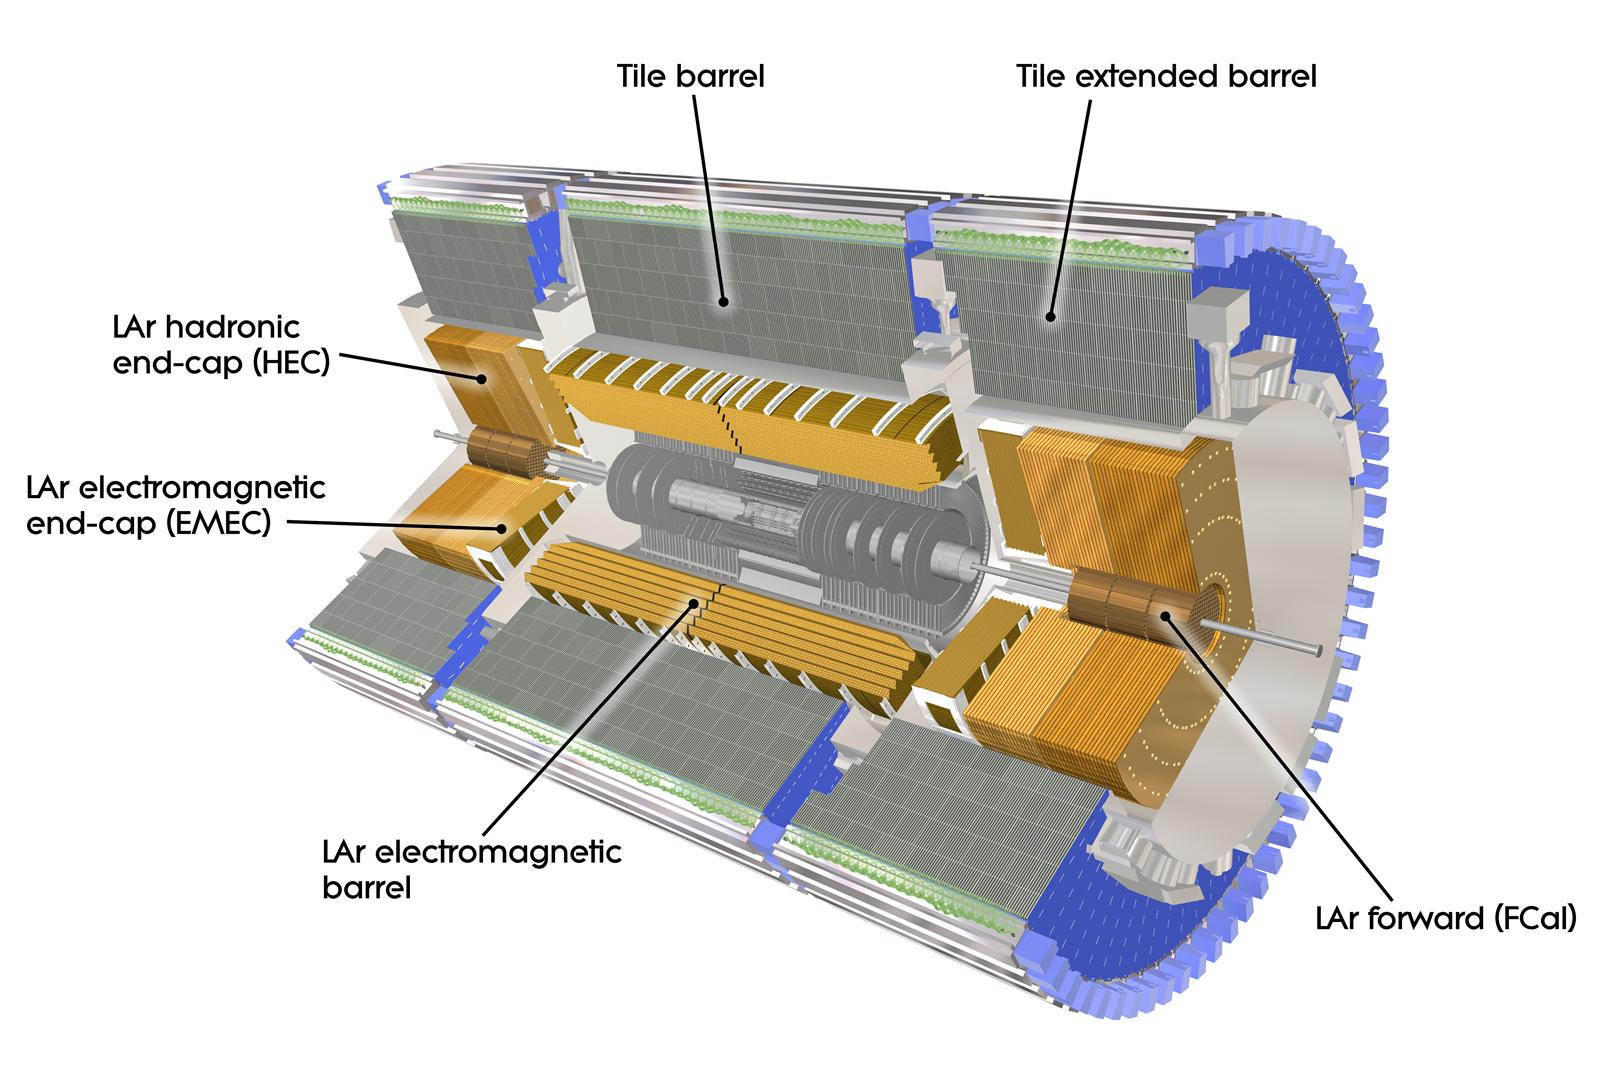
\includegraphics{figures/ch3-experiment/ATLAS_calorimeters_sketch}}
	\caption{A 3D model of the ATLAS calorimeters, showing the electromagnetic barrel and end-caps, hadronic barrel and end-caps, and the forward calorimeter.}
	\label{fig:ATLAS-calorimeters}
\end{figure}


\subsubsection{Electromagnetic Calorimeter}\label{sec:ATLAS-calorimeters-ecal}
% TO DO: Pictures!

The electromagnetic calorimeter consists of two half-barrels ($0<\eta<\pm1.475$) and two end-caps ($1.375<|\eta|<3.2$), all of which use LAr as the active material and steel-clad lead plates as the absorber. The lead plates are arranged in an accordion geometry to provide a uniform, gapless coverage in $\hat{\phi}$, shown for a barrel module in figure~\ref{fig:ATLAS-LAr-module}. The plates are interleaved with electrodes built from copper etchings on polymide. The outer conductive layers of the electrodes distribute the $2000~\mbox{V}$ high voltage over the electrode surface, which drifts the charges induced by ionization in the LAr towards the electrodes with a drift time of $450~\mbox{ns}$. The inner layer of the electrode, separated from the outer layers by isolating foils, collects the signals via capacitive coupling.

The two half-barrels occupy the region $2.8~\mbox{m}<R<4~\mbox{m}$ and $0~\mbox{m}<z<\pm3.2~\mbox{m}$. Each has 1024 lead plates with a thickness of $1.53~\mm$ for $|\eta|<0.8$ and $1.13~\mm$ for $|\eta|>0.8$. The barrels are divided into 16 modules, each covering an azimuthal angle of $\Delta \phi = 22.5^{\circ}$. Each module has three layers in depth to provide a rough measurement of the longitudinal profile of the electromagnetic showers. The segmentation of each layer in $\Delta\eta\times\Delta\phi$ is shown in table~\ref{table:ATLAS-LAr-segmentation}. The fine segmentation of the front layer, closest to the interaction point, aids particle identification and, in combination with the middle layer, allows for a reasonable measurement of photon trajectories.  

The end-caps, one on either side of the interaction region, measure $63~\cm$ in thickness with inner and outer radii of $33~\cm$ and $209.8~\cm$, respectively. Each end-cap contains two co-axial sub-wheels, divided by a $3~\mm$ gap at $|\eta|=2.5$. The inner and outer wheels contain 256 and 768 lead absorbers, respectively, with the same accordion geometry as used in the barrel.

% Material, dead material, and presampler design
The total amount of material before and in the electromagnetic calorimeters is shown in figure~\ref{fig:ATLAS-material-interaction-lengths} in terms of interaction lengths $X_0$. Note that 

% Conclusion
In total, the electromagnetic calorimeter has 101,760 readout channels for the barrel, 62,208 channels for the end-caps, 7,808 channels for the barrel presampler, and 1,536 channels for the end-cap presamplers. 

\begin{figure}
	LAr pictures
\end{figure}


\begin{table}[htbp]
	\centering
	\begin{tabular}{|l|c|c|}
		\hline
		Layer & $\eta$ range & Granularity $\Delta\eta\times\Delta\phi$ \\
		\hline
		Barrel presampler & $|\eta|<1.52$ & $0.025\times0.1$ \\
		\hline
		\multirow{2}{*}{Barrel 1} & $|\eta|<1.40$ & $0.025 / 8 \times 0.1$ \\
		 & $1.40<|\eta|<1.475$ & $0.025\times0.025$ \\
		\hline
		\multirow{2}{*}{Barrel 2} & $|\eta|<1.40$ & $0.025\times0.025$ \\
		 & $1.40<|\eta|<1.475$ & $0.075\times 0.025$ \\
		\hline
		Barrel 3 & $|\eta|<1.35$ & $0.050\times0.025$ \\
		\hline
		\hline
		\multirow{7}{*}{End-cap 1} & $1.375<|\eta|<1.425$ & $0.050\times0.1$ \\
		 & $1.425<|\eta|<1.5$ & $0.025\times0.1$ \\
		 & $1.5<|\eta|<1.8$ & $0.025/8\times0.1$ \\
		 & $1.8<|\eta|<2.0$ & $0.025/6\times0.1$ \\
		 & $2.0<|\eta|<2.4$ & $0.025/4\times0.1$ \\
		 & $2.4<|\eta|<2.5$ & $0.025\times0.1$ \\
		 & $2.5<|\eta|<3.2$ & $0.1\times0.1$ \\
		\hline
		\multirow{3}{*}{End-cap 2} & $1.375<|\eta|<1.425$ & $0.050\times0.025$ \\
		 & $1.425<|\eta|<2.5$ & $0.025\times0.025$ \\
		 & $2.5<|\eta|<3.2$ & $0.1\times0.1$ \\
		\hline
		End-cap 3 & $1.5<|\eta|<2.5$ & $0.050\times0.025$ \\
		\hline
	\end{tabular}
	\caption{Granularity of each layer of the LAr electromagnetic calorimeter.}
	\label{table:ATLAS-LAr-segmentation}
\end{table}





The calorimeter system surrounds the solenoid, and consists of electromagnetic and hadronic components. The electromagnetic calorimeter is a lead/liquid argon (LAr) sampling calorimeter, and comprises a barrel ($|\eta|<1.475$) and two endcaps ($1.375<|\eta|<3.2)$. In the range $|\eta|<2.5$, the detector is finely segmented in $\eta$ to provide good spatial resolution. The hadronic calorimeter (HCAL) uses steel/scintillator tiles in the barrel ($|\eta|<1.7$) and copper/LAr in the endcaps ($1.5<|\eta|<3.2$). In the forward region ($3.1<|\eta|<4.9$), electromagnetic and hadronic calorimetry is performed using copper/LAr and tungsten/LAr technology.



\subsubsection{Hadronic Calorimeter}\label{sec:ATLAS-calorimeters-hcal}


\subsubsection{Forward Calorimeter}\label{sec:ATLAS-calorimeters-fcal}



\subsection{Muon System}

\subsection{Data Acquisition}




\section{Data Taking}
\subsection{Performance during Run I}

\subsection{Luminosity Measurement}


\printbibliography